\documentclass[11pt,a4paper]{article}

\usepackage[utf8]{inputenc}
\usepackage[spanish]{babel}
\usepackage[T1]{fontenc}
\usepackage{geometry}
\geometry{margin=2.3cm}
\usepackage{hyperref}
\hypersetup{colorlinks=true, linkcolor=blue, urlcolor=blue}
\usepackage{longtable}
\usepackage{booktabs}
\usepackage{listings}
\usepackage{xcolor}
\usepackage{fancyhdr}
\usepackage{enumitem}
\usepackage{graphicx}
\usepackage{float}
\usepackage{caption}

\definecolor{riesgoAlto}{RGB}{178,34,34}
\definecolor{riesgoMedio}{RGB}{184,134,11}
\definecolor{riesgoBajo}{RGB}{46,125,50}
\newcommand{\riesgo}[1]{%
  \ifx#1A\textcolor{riesgoAlto}{\textbf{Alto}}\fi
  \ifx#1M\textcolor{riesgoMedio}{\textbf{Medio}}\fi
  \ifx#1B\textcolor{riesgoBajo}{\textbf{Bajo}}\fi
}

\lstset{
  basicstyle=\ttfamily\footnotesize,
  breaklines=true,
  backgroundcolor=\color{gray!8},
  frame=single,
  columns=fullflexible,
  showstringspaces=false
}

\pagestyle{fancy}
\fancyhf{}
\rhead{Hospital Management System}
\lhead{Informe Final -- V\&V de Software}
\rfoot{\thepage}

\begin{document}
\shorthandoff{"}
\sloppy
\emergencystretch=3em

% ============================================================
% CARATULA
% ============================================================
\begin{titlepage}
\centering
\vspace*{1cm}

{\Large \textbf{ESCUELA POLIT\'ECNICA NACIONAL}}\\[0.3cm]
{\large FACULTAD DE INGENIER\'IA DE SISTEMAS}\\[1.5cm]

\rule{\linewidth}{0.5pt}\\[0.4cm]
{\Large \textbf{PROYECTO FINAL}}\\[0.2cm]
{\Large \textbf{VALIDACI\'ON Y VERIFICACI\'ON DE SOFTWARE}}\\[0.4cm]
\rule{\linewidth}{0.5pt}\\[1.2cm]

{\huge \textbf{Hospital Management System}}\\[0.3cm]
{\large Informe Final Consolidado de Entregables}\\[0.2cm]
{\small (pruebas, an\'alisis est\'atico y an\'alisis de seguridad OWASP en un solo documento)}\\[2cm]

\begin{tabular}{rl}
\textbf{Integrantes:} & Erick Costa -- L\'ider Backend \\
                       & Jimmy Arias -- L\'ider Frontend \\
                       & Paul Salas -- L\'ider QA, Calidad y Seguridad \\[0.4cm]
\textbf{Profesor:}    & Christian Su\'arez \\[0.4cm]
\textbf{Asignatura:}  & Validaci\'on y Verificaci\'on de Software \\[0.4cm]
\textbf{Per\'iodo Acad\'emico:} & 2026A \\[0.4cm]
\textbf{Fecha:}       & 19 de julio de 2026 \\[0.4cm]
\textbf{Repositorio:} & \url{https://github.com/zeuspyEC/hospital-management}
\end{tabular}

\vfill
{\small Quito, Ecuador}
\end{titlepage}

\thispagestyle{fancy}
\tableofcontents
\newpage

% ============================================================
\section{Introducci\'on}

Este documento consolida, \textbf{en un solo informe}, todos los entregables
del proyecto final de Validaci\'on y Verificaci\'on de Software sobre el
\emph{Hospital Management System}: un sistema fullstack (Spring Boot 3.3 +
JavaScript vanilla + PostgreSQL 16) provisto como base por la c\'atedra, con
deficiencias intencionales que el grupo deb\'ia detectar mediante pruebas
sistem\'aticas, an\'alisis est\'atico y an\'alisis de seguridad.

Todo resultado presentado aqu\'i proviene de \textbf{ejecuciones reales} de
las herramientas correspondientes contra el c\'odigo y la aplicaci\'on en
ejecuci\'on (backend en \texttt{:8080}, frontend en \texttt{:3000},
PostgreSQL en Docker), el 19 de julio de 2026. Se incluyen capturas de
pantalla reales de la aplicaci\'on funcionando, de las vulnerabilidades
explotadas en vivo, y las salidas textuales completas de cada herramienta --
no se resume ni se omite evidencia.

Este informe describe \textbf{qu\'e se construy\'o y qu\'e resultado dio al
ejecutarlo}; la evaluaci\'on y calificaci\'on de cada entregable frente a la
r\'ubrica del curso corresponde al profesor.

\section{Distribuci\'on del equipo}

\begin{longtable}{@{}p{2.5cm}p{3cm}p{6.3cm}p{2cm}@{}}
\toprule
\textbf{Integrante} & \textbf{Rol} & \textbf{\'Areas de responsabilidad} & \textbf{Rama Git} \\
\midrule
\endhead
Erick Costa & L\'ider Backend &
  Configuraci\'on del backend, pruebas unitarias (JUnit 5 + Mockito),
  pruebas de integraci\'on (SpringBootTest + MockMvc + H2), correcci\'on de
  un bug real de serializaci\'on que romp\'ia \texttt{/api/citas} y
  \texttt{/api/historias-clinicas}. &
  \texttt{feature/backend-erick} \\
Jimmy Arias & L\'ider Frontend &
  Pruebas unitarias con Jest (\texttt{utils.js}, \texttt{api.js}), pruebas
  End-to-End con Playwright sobre los 4 flujos principales. &
  \texttt{feature/frontend-jimmy} \\
Paul Salas & L\'ider QA, Calidad y Seguridad &
  An\'alisis est\'atico (Checkstyle, SpotBugs + FindSecBugs, ESLint),
  an\'alisis de seguridad OWASP Top 10, documentaci\'on de hallazgos. &
  \texttt{feature/qa-paul} \\
\bottomrule
\end{longtable}

El flujo de ramas (\texttt{main} $\leftarrow$ \texttt{develop} $\leftarrow$
\texttt{feature/*}), las reglas de commit y el checklist de Pull Request
usados por el equipo est\'an definidos en
\texttt{.claude/skills/team-git-workflow/SKILL.md} y
\texttt{CONTRIBUTING.md}, ambos versionados en el repositorio.

\newpage
% ============================================================
\section{Arquitectura del sistema}

\begin{itemize}[nosep]
  \item \textbf{Backend:} Spring Boot 3.3.0, Spring Data JPA, Jakarta
    Validation, arquitectura en capas (\texttt{Controller} $\to$
    \texttt{Service} $\to$ \texttt{Repository}), con DTOs para la
    comunicaci\'on REST y un \texttt{GlobalExceptionHandler} centralizado.
  \item \textbf{Frontend:} JavaScript vanilla modular (\texttt{app.js},
    \texttt{api.js}, \texttt{utils.js} y un m\'odulo por entidad), sin
    bundler ni framework -- los objetos de cada m\'odulo se referencian
    desde atributos \texttt{onclick} en HTML generado din\'amicamente.
  \item \textbf{Base de datos:} PostgreSQL 16 en contenedor Docker, con
    \texttt{schema.sql}/\texttt{data.sql} de inicializaci\'on.
  \item \textbf{Entidades:} Paciente, Doctor, Cita (relaci\'on
    \texttt{@ManyToOne} a Doctor, pero \texttt{pacienteId} es solo una
    columna sin FK) e HistoriaClinica (relaciones a Paciente y Doctor).
\end{itemize}

\subsection*{Evidencia visual: aplicaci\'on en ejecuci\'on}

Capturas reales tomadas el 19 de julio de 2026 contra el sistema desplegado
localmente (\texttt{docker compose up -d} + \texttt{mvn spring-boot:run} +
frontend est\'atico en \texttt{:3000}).

\begin{figure}[H]
  \centering
  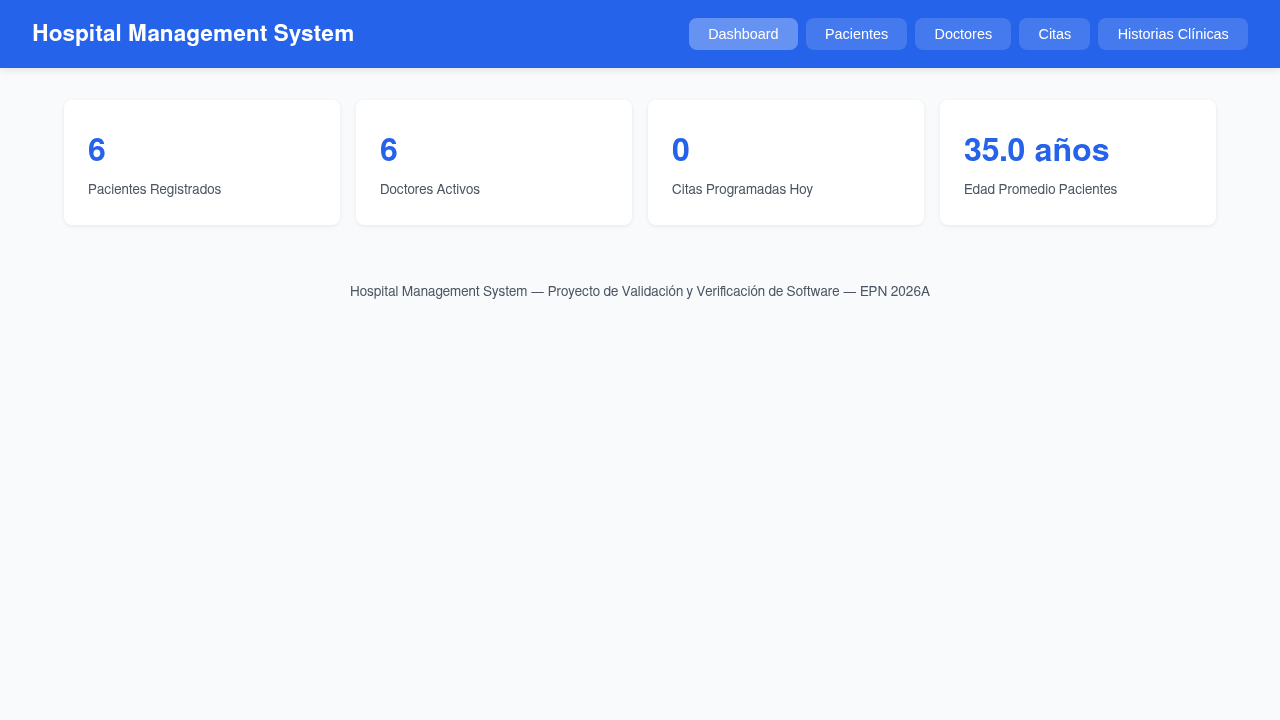
\includegraphics[width=0.95\linewidth]{img/01-dashboard.png}
  \caption{Dashboard mostrando contadores reales obtenidos de la API.}
\end{figure}

\begin{figure}[H]
  \centering
  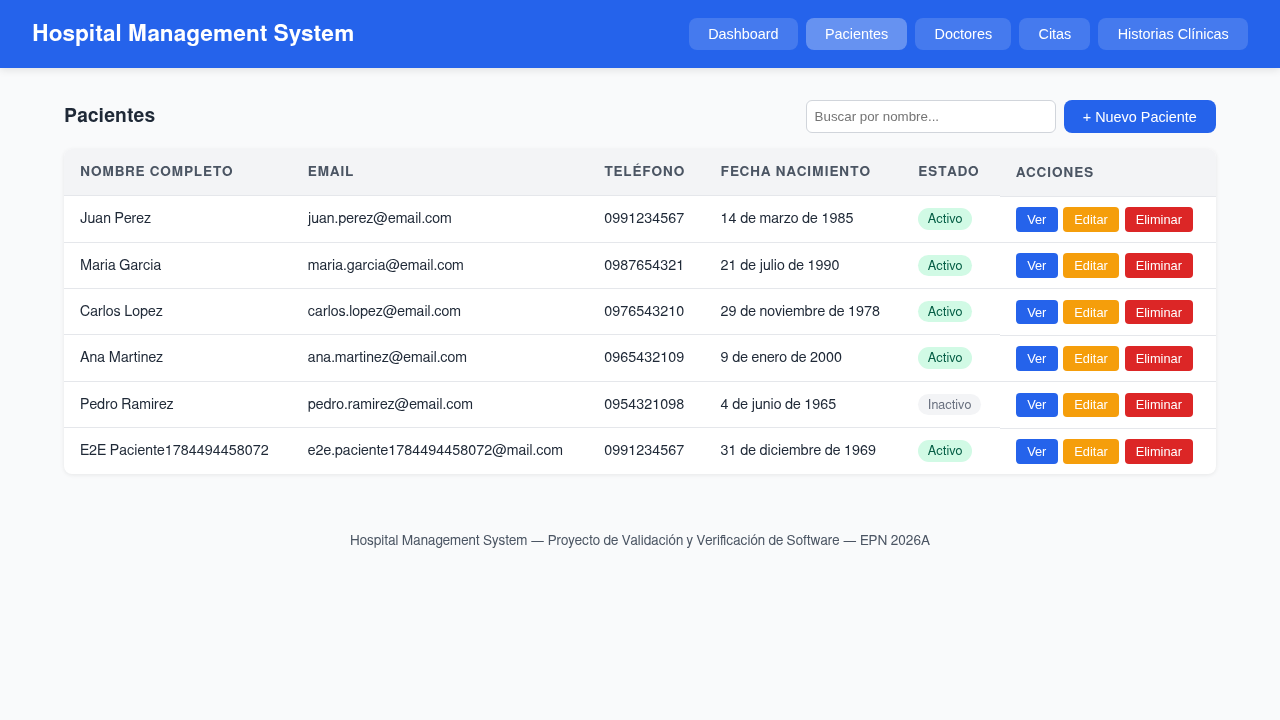
\includegraphics[width=0.95\linewidth]{img/02-pacientes.png}
  \caption{M\'odulo de Pacientes con datos precargados y registros creados
  durante las pruebas E2E.}
\end{figure}

\begin{figure}[H]
  \centering
  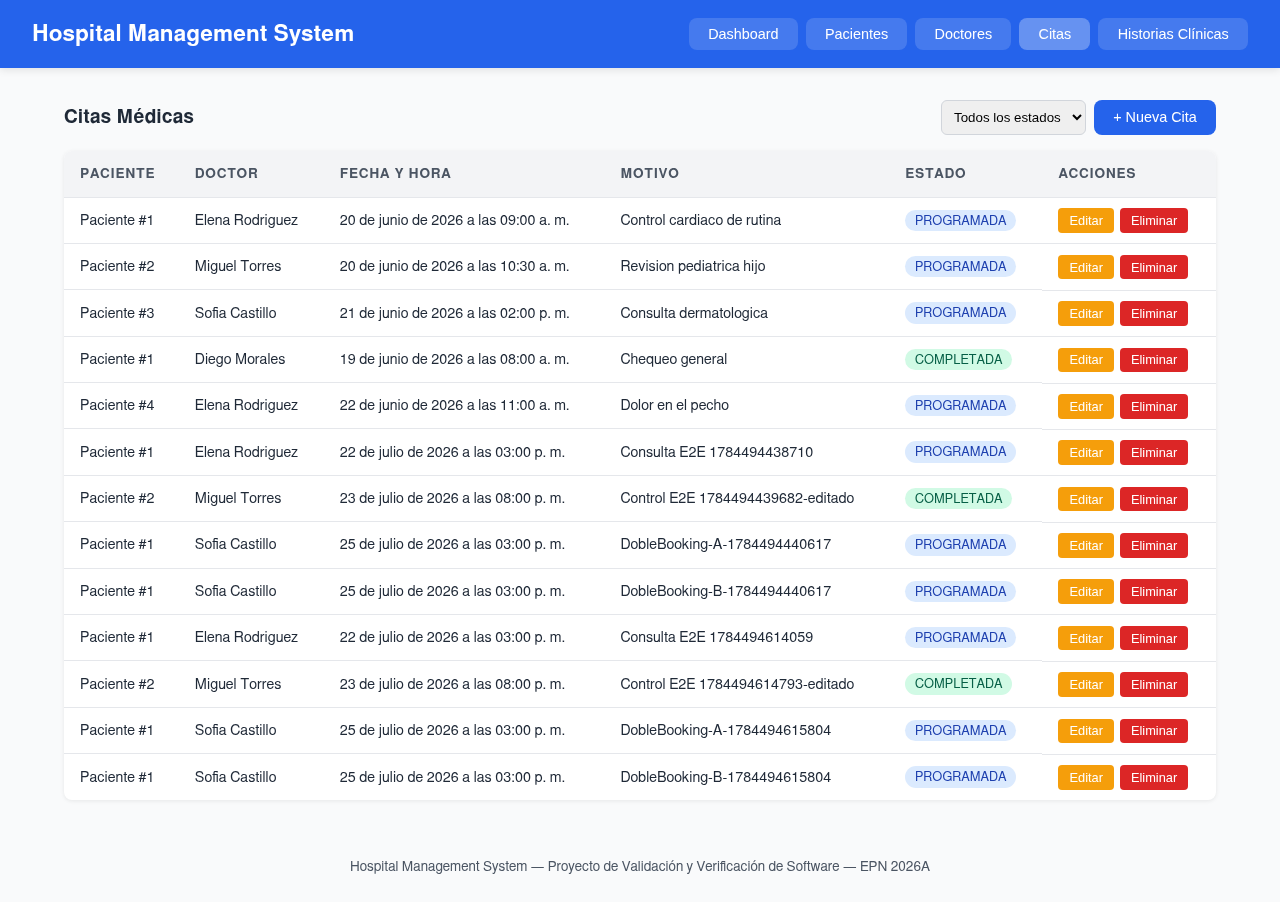
\includegraphics[width=0.95\linewidth]{img/04-citas.png}
  \caption{M\'odulo de Citas M\'edicas, incluyendo citas creadas por las
  pruebas de doble booking.}
\end{figure}

\section{Flujo de trabajo y control de versiones}

\begin{longtable}{@{}p{4cm}p{3cm}p{7cm}@{}}
\toprule
\textbf{Rama} & \textbf{Commits desde main} & \textbf{Contenido principal} \\
\midrule
\endhead
\texttt{feature/backend-erick} & 7 &
  4 clases de pruebas unitarias de servicio, 4 clases de integraci\'on de
  controlador, configuraci\'on de JaCoCo, correcci\'on del bug de
  serializaci\'on Jackson/Hibernate. \\
\texttt{feature/frontend-jimmy} & 8 &
  \texttt{utils.test.js}, \texttt{api.test.js}, 4 specs de Playwright,
  configuraci\'on de Jest/Playwright. \\
\texttt{feature/qa-paul} & 10+ &
  Configuraci\'on de Checkstyle/SpotBugs/ESLint, reportes crudos, este
  informe consolidado. \\
\bottomrule
\end{longtable}

\newpage
% ============================================================
\section{Pruebas Unitarias -- Backend}

\textbf{Herramientas:} JUnit 5 + Mockito. \textbf{Ubicaci\'on:}
\texttt{backend/src/test/java/com/hospital/service/}.

\begin{longtable}{@{}p{5.5cm}p{2cm}p{2cm}p{2cm}p{2cm}@{}}
\toprule
\textbf{Clase} & \textbf{Casos felices} & \textbf{Casos l\'imite} & \textbf{Errores} & \textbf{Total} \\
\midrule
\endhead
\texttt{PacienteServiceTest} & 5 & 3 & 4 & 12 \\
\texttt{DoctorServiceTest} & 5 & 3 & 2 & 10 \\
\texttt{CitaServiceTest} & 5 & 3 & 3 & 11 \\
\texttt{HistoriaClinicaServiceTest} & 5 & 2 & 3 & 10 \\
\midrule
\textbf{Total} & \textbf{20} & \textbf{11} & \textbf{12} & \textbf{43} \\
\bottomrule
\end{longtable}

\textbf{Salida real y completa de \texttt{mvn test} (JDK 17, 19 de julio de 2026):}
\begin{lstlisting}
[INFO] Running com.hospital.service.PacienteServiceTest$ManejoDeErrores
[INFO] Tests run: 4, Failures: 0, Errors: 0, Skipped: 0
[INFO] Running com.hospital.service.PacienteServiceTest$CasosLimite
[INFO] Tests run: 3, Failures: 0, Errors: 0, Skipped: 0
[INFO] Running com.hospital.service.PacienteServiceTest$CasosFelices
[INFO] Tests run: 5, Failures: 0, Errors: 0, Skipped: 0

[INFO] Running com.hospital.service.DoctorServiceTest$ManejoDeErrores
[INFO] Tests run: 2, Failures: 0, Errors: 0, Skipped: 0
[INFO] Running com.hospital.service.DoctorServiceTest$CasosLimite
[INFO] Tests run: 3, Failures: 0, Errors: 0, Skipped: 0
[INFO] Running com.hospital.service.DoctorServiceTest$CasosFelices
[INFO] Tests run: 5, Failures: 0, Errors: 0, Skipped: 0

[INFO] Running com.hospital.service.CitaServiceTest$ManejoDeErrores
[INFO] Tests run: 3, Failures: 0, Errors: 0, Skipped: 0
[INFO] Running com.hospital.service.CitaServiceTest$CasosLimite
[INFO] Tests run: 3, Failures: 0, Errors: 0, Skipped: 0
[INFO] Running com.hospital.service.CitaServiceTest$CasosFelices
[INFO] Tests run: 5, Failures: 0, Errors: 0, Skipped: 0

[INFO] Running com.hospital.service.HistoriaClinicaServiceTest$ManejoDeErrores
[INFO] Tests run: 3, Failures: 0, Errors: 0, Skipped: 0
[INFO] Running com.hospital.service.HistoriaClinicaServiceTest$CasosLimite
[INFO] Tests run: 2, Failures: 0, Errors: 0, Skipped: 0
[INFO] Running com.hospital.service.HistoriaClinicaServiceTest$CasosFelices
[INFO] Tests run: 5, Failures: 0, Errors: 0, Skipped: 0

[INFO] Results:
[INFO] Tests run: 43, Failures: 0, Errors: 0, Skipped: 0
[INFO] BUILD SUCCESS
\end{lstlisting}

Cada clase usa mocks de sus repositorios (\texttt{@Mock} +
\texttt{@ExtendWith(MockitoExtension.class)}) y est\'a organizada en tres
grupos \texttt{@Nested}: \texttt{CasosFelices}, \texttt{CasosLimite} y
\texttt{ManejoDeErrores}. Varios casos l\'imite reproducen expl\'icitamente
bugs intencionales del c\'odigo base (divisi\'on por cero en
\texttt{calcularEdadPromedio}, doble booking en citas, inyecci\'on SQL en
\texttt{buscarPorEspecialidadInsegura}, XSS almacenado sin sanitizar en
historias cl\'inicas).

\section{Pruebas de Integraci\'on -- Backend}

\textbf{Herramientas:} \texttt{@SpringBootTest} + MockMvc + H2 en memoria.
\textbf{Ubicaci\'on:} \texttt{backend/src/test/java/com/hospital/controller/}.

\begin{longtable}{@{}p{6cm}p{2.5cm}p{5cm}@{}}
\toprule
\textbf{Clase} & \textbf{Tests} & \textbf{Cobertura funcional} \\
\midrule
\endhead
\texttt{PacienteControllerIntegrationTest} & 9 & GET/POST/PUT/DELETE, validaci\'on, b\'usqueda \\
\texttt{DoctorControllerIntegrationTest} & 9 & GET/POST/PUT/DELETE, inyecci\'on SQL reproducida v\'ia HTTP \\
\texttt{CitaControllerIntegrationTest} & 11 & GET/POST/PUT/DELETE, doble booking, rango de fechas \\
\texttt{HistoriaClinicaControllerIntegrationTest} & 9 & GET/POST, XSS almacenado, validaci\'on \\
\midrule
\textbf{Total (unitarias + integraci\'on)} & \textbf{81} & \\
\bottomrule
\end{longtable}

\textbf{Salida real de \texttt{mvn test} (suite completa backend):}
\begin{lstlisting}
[INFO] Results:
[INFO] Tests run: 81, Failures: 0, Errors: 0, Skipped: 0
[INFO] BUILD SUCCESS
[INFO] Total time:  18.800 s
\end{lstlisting}

\textbf{Cobertura de c\'odigo (JaCoCo, generado con \texttt{mvn test jacoco:report}):}

\begin{longtable}{@{}p{4cm}p{2.5cm}p{2.5cm}@{}}
\toprule
\textbf{Paquete} & \textbf{Instrucciones} & \textbf{Ramas} \\
\midrule
\endhead
\texttt{com.hospital.service} & 97\% & 64\% \\
\texttt{com.hospital.controller} & 93\% & n/a \\
\texttt{com.hospital.model} & 98\% & n/a \\
\texttt{com.hospital.dto} & 100\% & n/a \\
\texttt{com.hospital.config} & 100\% & n/a \\
\texttt{com.hospital.exception} & 74\% & 100\% \\
\midrule
\textbf{Total del proyecto} & \textbf{95\%} & \textbf{68\%} \\
\bottomrule
\end{longtable}

\textbf{Bug real corregido durante esta fase (no intencional, no
documentado en comentarios del c\'odigo):} \texttt{GET /api/citas} y
\texttt{GET /api/historias-clinicas} devolv\'ian \texttt{500} de forma
consistente contra PostgreSQL real, por un
\texttt{InvalidDefinitionException} de Jackson al serializar proxies
Hibernate de relaciones \texttt{@ManyToOne(LAZY)}:
\begin{lstlisting}
$ curl -s http://localhost:8080/api/citas -o /dev/null -w "%{http_code}\n"
500
com.fasterxml.jackson.databind.exc.InvalidDefinitionException:
No serializer found for class
org.hibernate.proxy.pojo.bytebuddy.ByteBuddyInterceptor
\end{lstlisting}
Se agreg\'o el m\'odulo \texttt{jackson-datatype-hibernate6} con
\texttt{FORCE\_LAZY\_LOADING} (para no ocultar el bug intencional de
consultas N+1 que el enunciado pide detectar). Verificaci\'on posterior:
\begin{lstlisting}
$ curl -s http://localhost:8080/api/citas -o /dev/null -w "%{http_code}\n"
200
\end{lstlisting}

\newpage
% ============================================================
\section{Pruebas Unitarias -- Frontend}

\textbf{Herramientas:} Jest 29 + jsdom. \textbf{Ubicaci\'on:}
\texttt{frontend/js/\_\_tests\_\_/}.

\begin{longtable}{@{}p{5cm}p{2.5cm}p{2.5cm}p{4cm}@{}}
\toprule
\textbf{Archivo} & \textbf{Tests} & \textbf{Cobertura} & \textbf{Alcance} \\
\midrule
\endhead
\texttt{utils.test.js} & 32 & 100\% sentencias & Las 8 funciones exportadas de \texttt{utils.js} \\
\texttt{api.test.js} & 17 & 55\% sentencias & \texttt{apiFetch} + muestra de los 4 m\'odulos de API (fetch mockeado) \\
\midrule
\textbf{Total} & \textbf{49} & & \\
\bottomrule
\end{longtable}

\textbf{Salida real de \texttt{npx jest --coverage}:}
\begin{lstlisting}
PASS js/__tests__/utils.test.js
PASS js/__tests__/api.test.js
----------|---------|----------|---------|---------|
File      | % Stmts | % Branch | % Funcs | % Lines |
----------|---------|----------|---------|---------|
utils.js  |     100 |     90.9 |     100 |     100 |
----------|---------|----------|---------|---------|
Test Suites: 2 passed, 2 total
Tests:       49 passed, 49 total
\end{lstlisting}

\textbf{Bugs reales encontrados al ejecutar los tests} (contradicen los
comentarios "BUG INTENCIONAL" del propio c\'odigo fuente):
\begin{itemize}[nosep]
  \item \texttt{apiFetch} \textbf{pierde el header \texttt{Content-Type}}
    cuando se le pasan headers personalizados, porque
    \texttt{\{headers: \{...\}, ...options\}} hace que \texttt{options.headers}
    sobrescriba por completo el objeto ya fusionado.
  \item El regex de \texttt{validateEmail} \textbf{s\'i rechaza}
    \texttt{"usuario@dominio"} y \textbf{s\'i acepta} emails con \texttt{+},
    lo contrario de lo que afirma el comentario en el c\'odigo fuente.
\end{itemize}

\section{Pruebas E2E -- Frontend (Playwright)}

\textbf{Herramientas:} Playwright 1.47 (Chromium). \textbf{Ubicaci\'on:}
\texttt{frontend/e2e/}. Ejecutadas contra el \textbf{stack real completo}
(PostgreSQL en Docker, backend Spring Boot en \texttt{:8080}, frontend
est\'atico en \texttt{:3000}), no contra mocks.

\begin{longtable}{@{}p{5cm}p{2.5cm}p{6.5cm}@{}}
\toprule
\textbf{Archivo} & \textbf{Tests} & \textbf{Flujo cubierto} \\
\midrule
\endhead
\texttt{pacientes.spec.js} & 3 & CRUD completo, validaci\'on HTML5, b\'usqueda \\
\texttt{doctores.spec.js} & 3 & CRUD completo, especialidad opcional (bug), b\'usqueda \\
\texttt{citas.spec.js} & 4 & Creaci\'on/edici\'on, doble booking (bug), filtro por estado \\
\texttt{historias.spec.js} & 3 & Creaci\'on + consulta con "Ver", doctor opcional, XSS almacenado (bug) \\
\midrule
\textbf{Total} & \textbf{13} & \\
\bottomrule
\end{longtable}

\textbf{Salida real de \texttt{npx playwright test}:}
\begin{lstlisting}
Running 13 tests using 1 worker
  13 passed (10.3s)
\end{lstlisting}

\textbf{Hallazgo relevante encontrado durante la ejecuci\'on:} el DELETE de
pacientes y doctores \textbf{s\'i elimina el registro en el backend}
(\texttt{200} con cuerpo vac\'io), pero \texttt{apiFetch} intenta parsear ese
cuerpo vac\'io como JSON y lanza una excepci\'on; la UI muestra "Error al
eliminar" y \textbf{no refresca la tabla}, dejando una fila fantasma visible
aunque el registro ya no exista en la base de datos.

\newpage
% ============================================================
\section{An\'alisis Est\'atico de C\'odigo}

\subsection{Herramientas utilizadas y configuraci\'on}

\begin{longtable}{@{}p{2.6cm}p{3cm}p{5.5cm}p{2.5cm}@{}}
\toprule
\textbf{Herramienta} & \textbf{Alcance} & \textbf{Configuraci\'on} & \textbf{Invocaci\'on} \\
\midrule
\endhead
Checkstyle 3.5.0 & Backend (Java) & \texttt{google\_checks.xml} (Google Java
  Style), plugin agregado en \texttt{backend/pom.xml} &
  \texttt{mvn checkstyle:check} \\
SpotBugs 4.8.6.3 + FindSecBugs 1.13.0 & Backend (bytecode compilado) &
  \texttt{effort=Max}, \texttt{threshold=Low}, plugin de seguridad
  FindSecBugs agregado &
  \texttt{mvn spotbugs:spotbugs} \\
ESLint 8.57.1 & Frontend (\texttt{js/**/*.js}, \texttt{e2e/**/*.js}) &
  \texttt{eslint:recommended}, \texttt{.eslintrc.json} con
  \texttt{overrides} para tests (jest) y e2e (node) &
  \texttt{npx eslint "js/**/*.js" "e2e/**/*.js"} \\
\bottomrule
\end{longtable}

\subsection{Resumen de hallazgos por severidad}

\begin{longtable}{@{}p{4.2cm}p{2.6cm}p{2.6cm}p{2.6cm}p{1.8cm}@{}}
\toprule
\textbf{Herramienta} & \textbf{Blocker /\newline Alto} & \textbf{Critical /\newline Medio} & \textbf{Major /\newline Bajo} & \textbf{Total} \\
\midrule
\endhead
Checkstyle & 0 & 0 & 937 & \textbf{937} \\
SpotBugs + FindSecBugs & 0 & 9 (Medium) & 28 (Low) & \textbf{37} \\
ESLint & 0 & 0 & 4 (warning) & \textbf{4} \\
\midrule
\textbf{Total general} & \textbf{0} & \textbf{9} & \textbf{969} & \textbf{978} \\
\bottomrule
\end{longtable}

\subsection{Checkstyle -- desglose y salida real}

\begin{longtable}{@{}p{5cm}p{2cm}p{7cm}@{}}
\toprule
\textbf{Regla} & \textbf{Ocurrencias} & \textbf{Descripci\'on} \\
\midrule
\endhead
Indentation & 553 & El c\'odigo usa 4 espacios; Google Style exige 2. \\
RightCurlyAlone / LeftCurly & 224 & Estilo de llaves distinto al de Google. \\
EmptyLineSeparator & 56 & Faltan/sobran l\'ineas en blanco entre miembros de clase. \\
CustomImportOrder & 31 & Orden de imports incorrecto (ej. \texttt{java.util.List}
  debe ir antes que \texttt{org.springframework.*}). \\
MissingJavadocMethod / Type & 47 & Clases y m\'etodos p\'ublicos sin Javadoc. \\
LineLength & 13 & L\'ineas mayores a 100 caracteres. \\
AvoidStarImport & 8 & Imports con \texttt{*}. \\
AbbreviationAsWordInName & 4 & Nombres con abreviaciones (ej. \texttt{DTO}). \\
\bottomrule
\end{longtable}

\textbf{Salida real (fragmento) de \texttt{mvn checkstyle:check}:}
\begin{lstlisting}
[WARNING] src/main/java/com/hospital/service/DoctorService.java:[37,5]
  (indentation) Indentation: 'method def rcurly' esta en el nivel de
  sangrado 4, pero esto no es el nivel correcto. Se esperaba el nivel 2.
[WARNING] src/main/java/com/hospital/repository/PacienteRepository.java:[15]
  (sizes) LineLength: La linea es mayor de 100 caracteres (encontrado 105).
[WARNING] src/main/java/com/hospital/repository/HistoriaClinicaRepository.java:
  [9,1] (javadoc) MissingJavadocType: Falta el comentario Javadoc.
...
[INFO] You have 937 Checkstyle violations.
[INFO] BUILD SUCCESS
\end{lstlisting}

\textbf{Lectura:} el 96\% de las violaciones (777/937) son puramente de
formato y se resolver\'ian con un formateador autom\'atico
(\texttt{google-java-format}). Cero violaciones afectan la correcci\'on
funcional del c\'odigo.

\subsection{SpotBugs + FindSecBugs -- desglose y salida real}

\begin{longtable}{@{}p{3.5cm}p{1.7cm}p{1.5cm}p{6.5cm}@{}}
\toprule
\textbf{Patr\'on} & \textbf{Ocurrencias} & \textbf{Severidad} & \textbf{Descripci\'on} \\
\midrule
\endhead
SPRING\_ENDPOINT & 28 & Low & Informativo: marca cada m\'etodo p\'ublico de
  los 4 \texttt{@RestController} como endpoint expuesto. \\
EI\_EXPOSE\_REP2 & 6 & Medium & \texttt{Cita}/\texttt{HistoriaClinica}
  guardan referencias directas a objetos mutables (\texttt{Doctor},
  \texttt{Paciente}) sin copiarlos. \\
EI\_EXPOSE\_REP & 3 & Medium & Los getters devuelven la referencia interna
  mutable directamente. \\
\bottomrule
\end{longtable}

\textbf{Salida real de \texttt{mvn spotbugs:check} (fragmento):}
\begin{lstlisting}
[ERROR] Medium: com.hospital.model.Cita.getDoctor() may expose internal
  representation by returning Cita.doctor [com.hospital.model.Cita]
  At Cita.java:[line 51] EI_EXPOSE_REP
[ERROR] Medium: new com.hospital.model.HistoriaClinica(Paciente, Doctor,
  String, String, String) may expose internal representation by storing
  an externally mutable object into HistoriaClinica.paciente
  At HistoriaClinica.java:[line 38] EI_EXPOSE_REP2
[INFO] BUILD SUCCESS
\end{lstlisting}

\textbf{Nota metodol\'ogica importante (falso negativo):} SpotBugs +
FindSecBugs, con la configuraci\'on m\'as sensible disponible
(\texttt{effort=Max}, \texttt{threshold=Low}), \textbf{no detect\'o} la
inyecci\'on SQL real en \texttt{DoctorService.buscarPorEspecialidadInsegura}.
Esa vulnerabilidad solo se evidenci\'o con pruebas de integraci\'on
dirigidas y, como se muestra en la Secci\'on~11, explot\'andola en vivo desde
el navegador. Es la lecci\'on metodol\'ogica central de este an\'alisis: el
an\'alisis est\'atico gen\'erico no reemplaza las pruebas de seguridad
dirigidas.

\subsection{ESLint -- desglose y salida real}

\begin{lstlisting}
frontend/js/citas.js
  11:7  warning  'CitasModule' is assigned a value but never used

frontend/js/doctores.js
  10:7  warning  'DoctoresModule' is assigned a value but never used

frontend/js/historias.js
  10:7  warning  'HistoriasModule' is assigned a value but never used

frontend/js/pacientes.js
  11:7  warning  'PacientesModule' is assigned a value but never used

4 problems (0 errors, 4 warnings)
\end{lstlisting}

Los 4 warnings son \textbf{falsos positivos} propios de la arquitectura sin
bundler: cada objeto \texttt{XModule} se usa exclusivamente desde atributos
\texttt{onclick="..."} dentro de cadenas HTML generadas din\'amicamente, algo
que ESLint no puede rastrear en el AST de JavaScript. No representan c\'odigo
muerto real.

\subsection{An\'alisis de hallazgos relevantes de est\'atico (m\'inimo 5 requerido)}

\begin{enumerate}[leftmargin=*]
  \item \textbf{Indentation (553 casos):} adoptar Google Style de forma
    retroactiva tocar\'ia pr\'acticamente cada archivo; conviene decidir el
    est\'andar \emph{antes} de escribir m\'as c\'odigo.
  \item \textbf{MissingJavadocMethod/Type (47 casos):} ninguna clase p\'ublica
    del backend tiene Javadoc, incluyendo los repositorios con \texttt{@Query}
    personalizado donde un comentario evitar\'ia confusiones como la del
    punto 6 de esta lista.
  \item \textbf{EI\_EXPOSE\_REP2 en \texttt{HistoriaClinica}:} expone
    directamente \texttt{Paciente} y \texttt{Doctor}, entidades con datos
    sanitarios/personales.
  \item \textbf{Falso negativo de SpotBugs en la inyecci\'on SQL real:} el
    hallazgo metodol\'ogicamente m\'as importante de todo el an\'alisis
    est\'atico.
  \item \textbf{ESLint "limpio" $\neq$ ausencia de XSS:} los hallazgos XSS
    reales (m\'ultiples usos de \texttt{innerHTML} sin escapar) no son
    detectables por \texttt{eslint:recommended} sin un plugin de seguridad
    espec\'ifico (ej. \texttt{eslint-plugin-no-unsanitized}), no configurado
    en este proyecto.
  \item \textbf{CustomImportOrder id\'entico en los 4 repositorios (31
    casos):} sugiere que se generaron desde la misma plantilla -- buen
    candidato para \texttt{.editorconfig} + formateador en pre-commit.
\end{enumerate}

\newpage
% ============================================================
\section{An\'alisis de Seguridad -- OWASP Top 10 (2021)}

Se identificaron \textbf{11 hallazgos}, todos verificados de forma
reproducible (petici\'on HTTP real, captura de pantalla de la explotaci\'on
en vivo, o test automatizado en verde), mapeados a 6 categor\'ias.

\begin{longtable}{@{}p{0.6cm}p{6.5cm}p{3cm}p{1.8cm}@{}}
\toprule
\textbf{\#} & \textbf{Hallazgo} & \textbf{Categor\'ia} & \textbf{Riesgo} \\
\midrule
\endhead
1 & Ausencia total de autenticaci\'on/autorizaci\'on & A01:2021 & \riesgo{A} \\
2 & CORS permisivo (\texttt{origins="*"}) & A01:2021 & \riesgo{M} \\
3 & Credenciales de BD en texto plano en el repositorio & A02:2021 & \riesgo{A} \\
4 & Inyecci\'on SQL real (b\'usqueda de doctores) & A03:2021 & \riesgo{A} \\
5 & XSS almacenado en historias cl\'inicas & A03:2021 & \riesgo{A} \\
6 & XSS por \texttt{innerHTML} en Pacientes/Doctores/Citas & A03:2021 & \riesgo{M} \\
7 & XSS en \texttt{showAlert()} (compartido por todos los m\'odulos) & A03:2021 & \riesgo{M} \\
8 & Componentes desactualizados (Spring Boot 3.3.0 $\to$ 4.1.0) & A06:2021 & \riesgo{M} \\
9 & C\'odigos HTTP incorrectos (200 en vez de 404/201/204) & A05:2021 & \riesgo{M} \\
10 & Exposici\'on de stack traces completos en errores 500 & A05:2021 & \riesgo{M} \\
11 & Sin logging del servidor ante errores no controlados & A09:2021 & \riesgo{A} \\
\bottomrule
\end{longtable}

\subsection*{Hallazgo 4 (A03:2021) -- Inyecci\'on SQL real: explotada en vivo}

\textbf{Ubicaci\'on:} \texttt{DoctorService.java:57-61}
(\texttt{buscarPorEspecialidadInsegura}), expuesta en
\texttt{DoctorController.java:52} y consumida directamente por el buscador
del m\'odulo Doctores en el frontend (\texttt{DoctoresAPI.buscarPorEspecialidad}
en \texttt{api.js}):
\begin{lstlisting}[language=java]
String sql = "SELECT * FROM doctores WHERE especialidad ILIKE '%"
             + especialidad + "%'";
Query query = entityManager.createNativeQuery(sql, Doctor.class);
\end{lstlisting}

\textbf{Evidencia paso 1 -- b\'usqueda normal (0 resultados esperados):}
\begin{figure}[H]
  \centering
  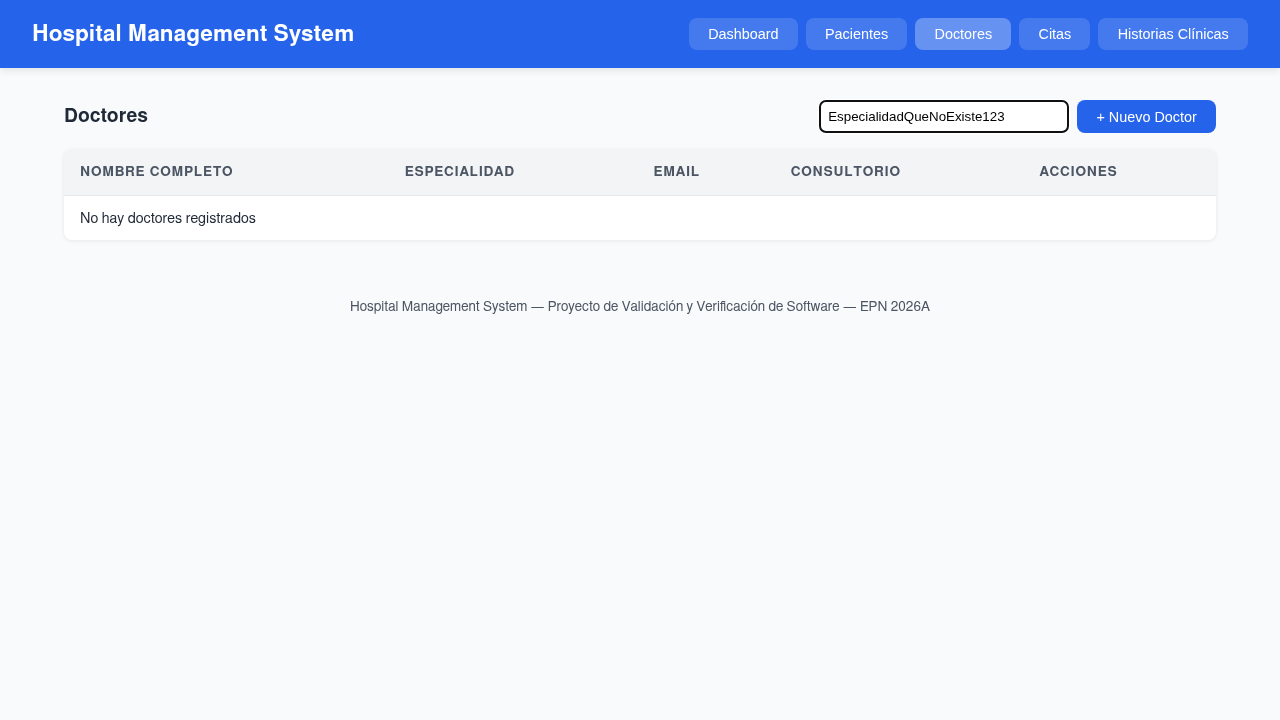
\includegraphics[width=0.95\linewidth]{img/07-sqli-busqueda-normal.png}
  \caption{Buscar "EspecialidadQueNoExiste123" filtra correctamente: 0 doctores.}
\end{figure}

\textbf{Evidencia paso 2 -- payload \texttt{' OR '1'='1' -- } en el MISMO
cuadro de b\'usqueda de la interfaz (sin herramientas externas, solo
tipeando en el navegador):}
\begin{figure}[H]
  \centering
  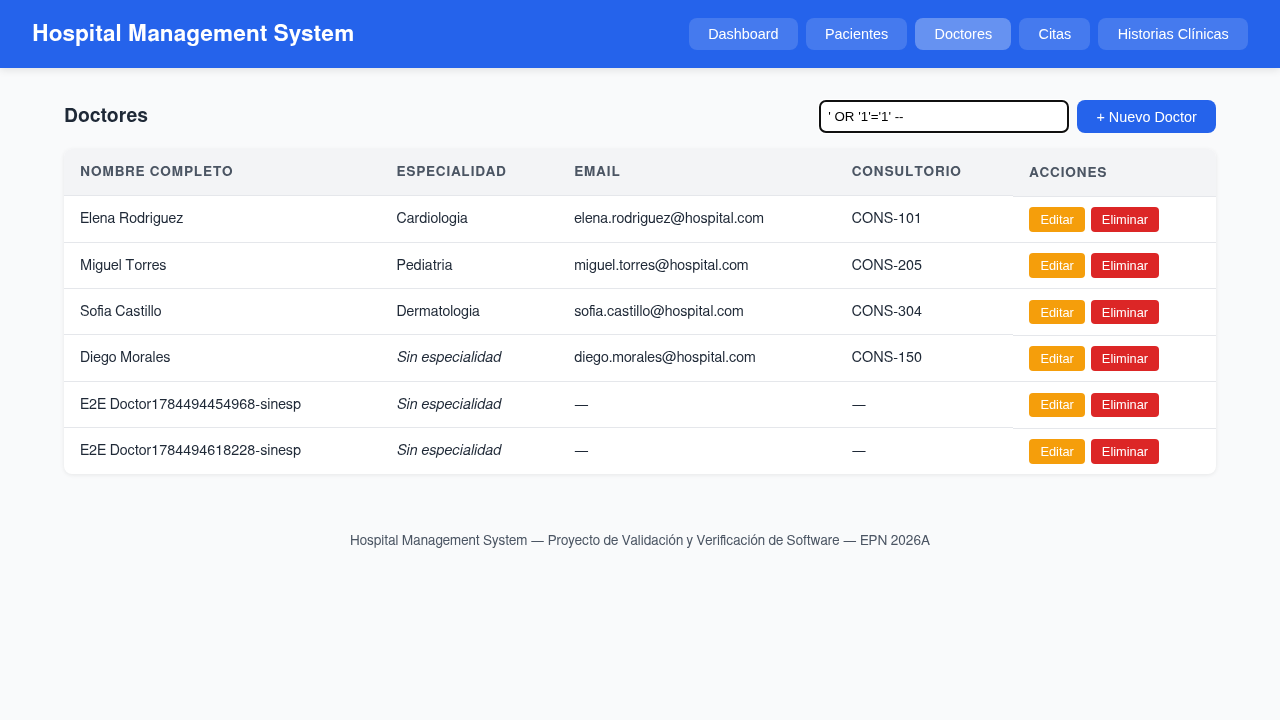
\includegraphics[width=0.95\linewidth]{img/08-sqli-inyeccion-real.png}
  \caption{El filtro queda completamente anulado: se devuelven TODOS los
  doctores de la base de datos, ignorando la especialidad buscada. Inyecci\'on
  SQL confirmada end-to-end, desde la UI real.}
\end{figure}

\textbf{Impacto:} cualquier usuario del formulario de b\'usqueda de doctores
-- sin conocimientos t\'ecnicos avanzados, sin herramientas de intercepci\'on
-- puede alterar la l\'ogica de la consulta SQL. \textbf{Mitigaci\'on:}
eliminar \texttt{buscarPorEspecialidadInsegura} y usar exclusivamente
\texttt{buscarPorEspecialidad} (ya existente, con par\'ametros ligados por
Spring Data).

\subsection*{Hallazgo 5 (A03:2021) -- XSS almacenado: explotado en vivo}

\textbf{Ubicaci\'on:} \texttt{HistoriaClinicaService.java} (no sanitiza al
guardar) + \texttt{frontend/js/historias.js:53} (\texttt{renderTabla} usa
\texttt{innerHTML} con datos del backend sin escapar).

\textbf{Evidencia -- historia cl\'inica creada con diagn\'ostico
\texttt{<b style="color:red">EVIDENCIA XSS: esto deberia verse como texto
plano, no en negrita/rojo</b>} desde el formulario real de la aplicaci\'on:}
\begin{figure}[H]
  \centering
  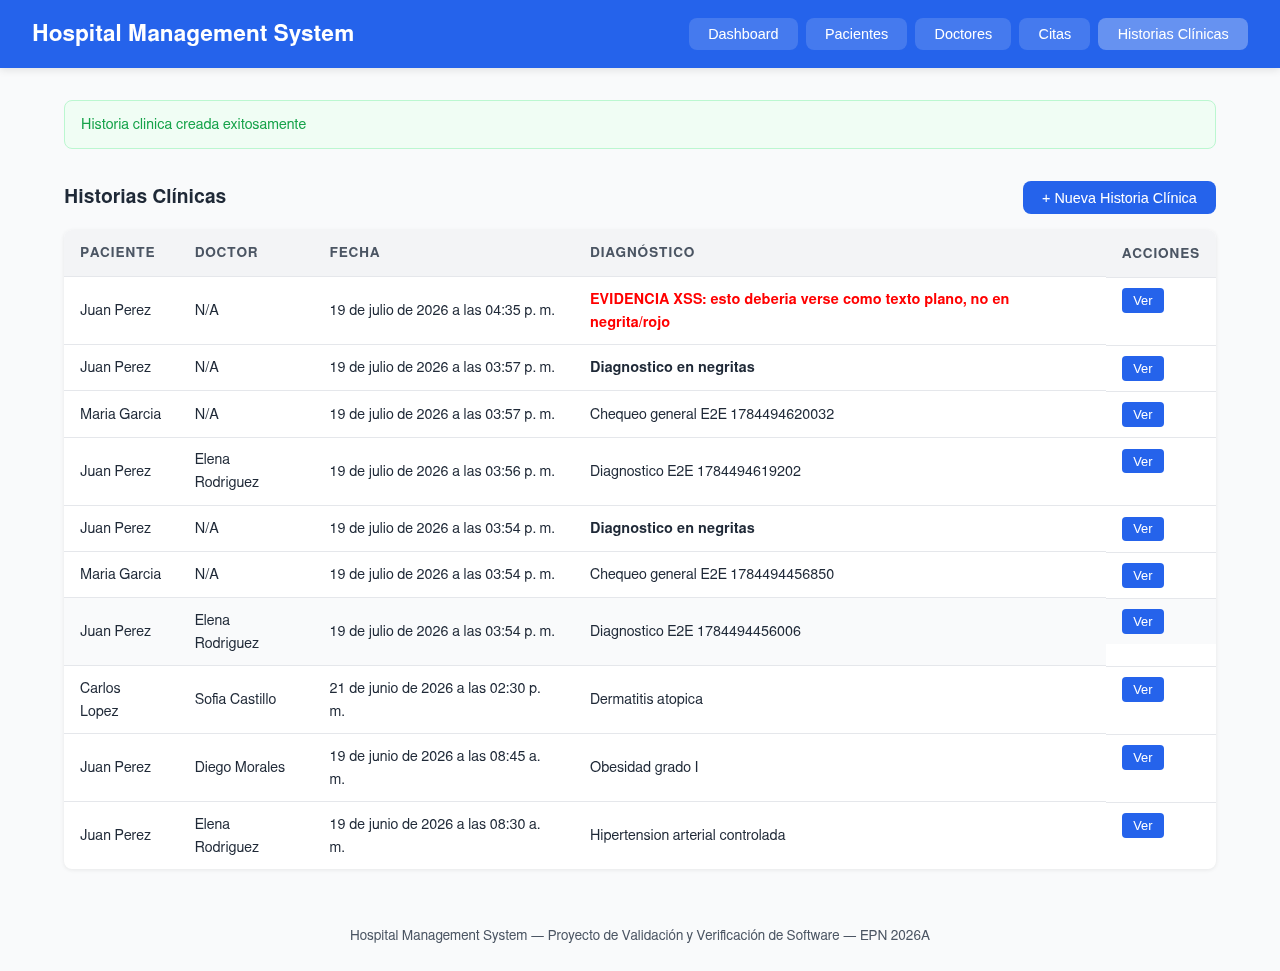
\includegraphics[width=0.95\linewidth]{img/06-xss-evidencia.png}
  \caption{El texto se renderiza en \textbf{negrita y rojo real}: el
  navegador interpret\'o el HTML inyectado como marcado v\'alido, no como
  texto plano. Si estuviera escapado correctamente, se ver\'ia literalmente
  \texttt{<b style="color:red">...</b>} como texto.}
\end{figure}

\textbf{Impacto:} cualquier campo de diagn\'ostico puede contener
\texttt{<script>} o manejadores de evento (\texttt{onerror}, etc.) que se
ejecutan en el navegador de cualquiera que consulte esa historia cl\'inica
-- incluyendo personal m\'edico. \textbf{Mitigaci\'on:} usar
\texttt{textContent} en vez de \texttt{innerHTML}, o sanitizar con
\texttt{escapeHTML()} (corrigiendo tambi\'en esa funci\'on, que actualmente
no escapa comillas simples ni backticks).

\subsection*{Resto de hallazgos}

Los hallazgos 1, 2, 3, 6, 7, 8, 9, 10 y 11 -- con ubicaci\'on exacta,
impacto, evidencia de reproducci\'on (peticiones \texttt{curl}, salidas de
tests) y mitigaci\'on recomendada para cada uno -- se detallan a
continuaci\'on:

\begin{description}[leftmargin=1.2cm,style=nextline]
  \item[Hallazgo 1 -- A01:2021, Alto.] Ninguna dependencia de Spring
    Security ni entidad de usuario en todo el proyecto. Cualquier cliente
    an\'onimo lista/crea/modifica/elimina cualquier recurso. Verificado con
    \texttt{curl} sin header \texttt{Authorization} en cualquier endpoint.
  \item[Hallazgo 2 -- A01:2021, Medio.] \texttt{@CrossOrigin(origins = "*")}
    en los 4 controladores (\texttt{PacienteController.java:14},
    \texttt{DoctorController.java:14}, \texttt{CitaController.java:15},
    \texttt{HistoriaClinicaController.java:14}). Confirmado con
    \texttt{curl -H "Origin: https://sitio-malicioso.example"}, que
    devuelve ese mismo origen en \texttt{Access-Control-Allow-Origin}.
  \item[Hallazgo 3 -- A02:2021, Alto.]
    \texttt{application.properties:7-8} tiene
    \texttt{spring.datasource.password=hospital123} en texto plano,
    versionado en git. Verificable con
    \texttt{git show HEAD:backend/src/main/resources/application.properties}.
  \item[Hallazgo 6 -- A03:2021, Medio.] El mismo patr\'on de
    \texttt{innerHTML} sin escapar del Hallazgo 5 se repite en
    \texttt{pacientes.js:51}, \texttt{doctores.js:35} y \texttt{citas.js:54}.
  \item[Hallazgo 7 -- A03:2021, Medio.] \texttt{utils.js:71}:
    \texttt{container.innerHTML = `<div class="alert alert-\$\{type\}">\$\{message\}</div>`;}
    -- confirmado con \texttt{utils.test.js}, que verifica que un payload
    \texttt{<img src=x onerror=...>} se inserta sin convertirse a entidades HTML.
  \item[Hallazgo 8 -- A06:2021, Medio.] Spring Boot 3.3.0 vs. 4.1.0
    disponible; PostgreSQL driver 42.7.3 vs. 42.7.13. Verificado con
    \texttt{mvn versions:display-dependency-updates}.
  \item[Hallazgo 9 -- A05:2021, Medio.] \texttt{GlobalExceptionHandler.java:25}
    responde \texttt{ResponseEntity.ok(body)} para "no encontrado" (status
    HTTP real 200, no 404); POST devuelve 200 en vez de 201; DELETE 200 en
    vez de 204. Confirmado con las 4 clases de
    \texttt{*ControllerIntegrationTest}.
  \item[Hallazgo 10 -- A05:2021, Medio.]
    \texttt{GlobalExceptionHandler.java:54}: \texttt{body.put("stackTrace",
    ex.getStackTrace())} expone la traza completa al cliente en cualquier
    error 500 (reproducido en vivo antes de la correcci\'on de la
    Secci\'on~7).
  \item[Hallazgo 11 -- A09:2021, Alto.] El manejador gen\'erico de
    excepciones \textbf{nunca llama a un logger}. Descubierto de primera
    mano depurando el bug de la Secci\'on~7: el error 500 en
    \texttt{/api/citas} no dej\'o \textbf{ninguna} l\'inea en los logs del
    servidor pese a fallar en cada intento.
\end{description}

\subsection*{Priorizaci\'on de hallazgos OWASP}

\begin{enumerate}[nosep]
  \item \textbf{Cr\'itico:} Hallazgos 1, 3, 4 y 11 -- combinados, permiten a
    cualquier persona externa leer y modificar historiales cl\'inicos
    completos sin dejar rastro.
  \item \textbf{Alto valor / bajo esfuerzo:} Hallazgos 9 y 10 son
    correcciones de una l\'inea cada una en \texttt{GlobalExceptionHandler.java}.
  \item \textbf{Transversal:} Hallazgos 5, 6 y 7 comparten la misma causa
    ra\'iz (falta de escape sistem\'atico al insertar en el DOM) y se
    resuelven con un solo cambio consistente en los 4 m\'odulos frontend.
\end{enumerate}

\newpage
% ============================================================
\section{Resumen consolidado de ejecuci\'on}

\begin{longtable}{@{}p{6cm}p{2.5cm}p{2.5cm}p{3cm}@{}}
\toprule
\textbf{Suite} & \textbf{Tests} & \textbf{Resultado} & \textbf{Comando} \\
\midrule
\endhead
Unitarias backend (JUnit 5 + Mockito) & 43 & 0 fallos & \texttt{mvn test -Dtest=*ServiceTest} \\
Integraci\'on backend (SpringBootTest + H2) & 38 (81 total con unitarias) & 0 fallos & \texttt{mvn test -Dtest=*ControllerIntegrationTest} \\
Unitarias frontend (Jest) & 49 & 0 fallos & \texttt{npx jest} \\
E2E frontend (Playwright) & 13 & 0 fallos & \texttt{npx playwright test} \\
\midrule
\textbf{Total pruebas automatizadas} & \textbf{143} & \textbf{0 fallos} & \\
\bottomrule
\end{longtable}

\begin{longtable}{@{}p{6cm}p{2.5cm}p{6cm}@{}}
\toprule
\textbf{Herramienta de an\'alisis} & \textbf{Hallazgos} & \textbf{Aporte principal} \\
\midrule
\endhead
Checkstyle & 937 & Deuda de formato/documentaci\'on (Google Java Style) \\
SpotBugs + FindSecBugs & 37 & Exposici\'on de representaci\'on interna; \emph{falso negativo} en SQLi \\
ESLint & 4 & Falsos positivos estructurales (arquitectura sin bundler) \\
OWASP Top 10 (an\'alisis dirigido) & 11 & Los hallazgos de mayor impacto real del proyecto \\
\bottomrule
\end{longtable}

\section{Bugs reales encontrados no documentados en el enunciado}

Adem\'as de los bugs intencionales del enunciado (que las pruebas de las
secciones anteriores reproducen sistem\'aticamente), el equipo encontr\'o y
document\'o los siguientes defectos \textbf{no anunciados} en los
comentarios del c\'odigo base:

\begin{enumerate}[nosep]
  \item \texttt{GET /api/citas} y \texttt{GET /api/historias-clinicas}
    romp\'ian por completo (500) contra PostgreSQL real -- corregido
    (Secci\'on 7).
  \item \texttt{apiFetch} pierde el header \texttt{Content-Type} al recibir
    headers personalizados.
  \item El comentario "BUG INTENCIONAL" de \texttt{validateEmail} describe
    un comportamiento que el regex real no tiene.
  \item El comentario "BUG INTENCIONAL" de
    \texttt{PacienteRepository.buscarPorNombre} afirma que la query es
    vulnerable a inyecci\'on SQL, pero usa \emph{binding} parametrizado
    (\texttt{:nombre}) correctamente -- no es explotable, a diferencia del
    m\'etodo de \texttt{DoctorService} que s\'i lo es (Secci\'on 11).
  \item El DELETE de pacientes/doctores deja una fila fantasma en la UI
    (Secci\'on 9).
\end{enumerate}

\section{Estructura de entregables en el repositorio}

\begin{lstlisting}
hospital-management/
|-- backend/src/test/java/com/hospital/
|   |-- service/              (4 clases, 43 tests)
|   `-- controller/            (4 clases, integracion con H2)
|-- frontend/
|   |-- js/__tests__/          (utils.test.js, api.test.js)
|   `-- e2e/                   (4 specs de Playwright)
|-- informes/
|   |-- analisis-estatico.pdf  (version independiente de la Seccion 8)
|   `-- analisis-owasp.pdf     (version independiente de la Seccion 9)
|-- docs/
|   |-- informes/              (reportes crudos: checkstyle, spotbugs, eslint)
|   `-- informe-final/         (este documento, con capturas en img/)
|-- .claude/skills/team-git-workflow/SKILL.md
|-- CONTRIBUTING.md
`-- .github/PULL_REQUEST_TEMPLATE.md
\end{lstlisting}

\section{Reproducibilidad}

Todos los resultados de este informe pueden reproducirse con:

\begin{lstlisting}[language=bash]
# Base de datos
docker compose up -d

# Backend (requiere JDK 17)
cd backend && mvn test                 # 81 tests
mvn spotbugs:spotbugs && mvn checkstyle:check

# Frontend
cd frontend && npm install
npx jest --coverage                    # 49 tests
npx eslint "js/**/*.js" "e2e/**/*.js"

# E2E (requiere backend + frontend + DB arriba)
npx playwright install chromium
npx playwright test                    # 13 tests
\end{lstlisting}

\section*{Nota final}

Este informe presenta \'unicamente resultados obtenidos de ejecutar
herramientas reales contra el c\'odigo y la aplicaci\'on: conteos de tests,
salidas de consola, capturas de pantalla de vulnerabilidades explotadas en
vivo. No incluye autoevaluaci\'on ni puntajes contra la r\'ubrica del curso
-- esa evaluaci\'on corresponde al profesor.

\end{document}
